\chapter{Objetivos}

Investigar como mutações identificadas no estado do Amazonas e no mundo para o HPV-16 podem interferir no reconhecimento de proteínas supressoras de tumor.

\section{Objetivos específicos}

\begin{enumerate}
    \item Modelar a estrutura tridimensional das proteínas E6 e E7 usando o AlphaFold tanto para forma ausente de mutações quanto para as mutações L90V, H85Y e Q21H para E6. Além da inserção das mutações G43E e G43E para E7 encontradas no Amazonas, e outras a nível mundial;

    \item Realizar o docking molecular usando o AlphaFold com proteínas supressores de tumor p53 e P16INK4a;

    \item Simular a dinâmica molecular ao longo de 200 ns (nanossegundos) da interação do complexo E6/E7 com as proteínas supressoras;

    \item Predição de epítopos antigênicos e primers dos segmentos E6 e E7 e avaliar a interação com anticorpos neutralizantes para o desenvolvimento de novos diagnósticos rápidos para HPV-16;

    \item Disponibilizar publicamente os dados obtidos no Github, criando uma base de dados acessível.
\end{enumerate}

\part{Materiais e Métodos}

% ----------------------------------------------------------
% Este capítulo, utilizado por diferentes exemplos do abnTeX2, ilustra o uso de
% comandos do abnTeX2 e de LaTeX.
% ----------------------------------------------------------

\chapter{Materiais e Métodos}\label{cap_exemplos}

\section{Modelagem estrutural das mutações}

O sequenciamento genético da forma ausente de mutações (wild-type) será obtida pela plataforma NCBI pelo código NC\_001526 referente ao HPV-16, onde a transcrição para o segmento E6 e E7 já é fornecida. A partir das mutações já descobertas e publicadas na literatura, entre estas a H85Y e  será feita a predição estrutural por um algoritmo de deep-learning, uma técnica avançada de IA utilizando o servidor do AlphaFold (https://alphafoldserver.com/). Os dados de entrada consistirão basicamente na sequência de aminoácidos do segmento E6 e E7, ao interagir com proteínas supressores de tumor, dentre estas p53. 

As estruturas foram validadas pelo mapa de contato gerado na própria ferramenta fornecendo um score e também pela plataforma MolProbity. Além disso, serão empregados estruturas já resolvidas experimentalmente por técnicas cristalográficas depositadas na base de dados Protein Data Bank, incluindo a interação p53-E6-E6AP sob o código de PDB ID: 4XR8 (Zapien et al, 2016). Além disso, será analisado como os anticorpos neutralizante V5 e U4 agem com a proteína L1 do capsídeo do HPV-16 sob o código PDB ID: 6BT3 (Guan et al, 2017).

\section{Predição de epítopos antigênicos}

A predição de epítopos antigênicos tanto para os segmentos L1/L2 quanto E6/E7 será realizada com base nas mutações detectadas no Amazonas, no Brasil e no mundo. Será empregado a ferramenta IEDB-MHC-I (https://www.iedb.org/) bem como IEDB-T-Cell que faz uso de redes neurais artificiais (VITA et al, 2025), um subtipo de IA, em diferentes alelos HLA. Os epítopos gerados serão modelados usando o AlphaFold e posteriormente feito o docking com receptor de células-T e Toll-like receptor II (TLR2) para avaliação da imunogenicidade.

\section{Docking molecular do tipo proteína-proteína}

As sequências de aminoácidos de referência (wild-type) para as oncoproteínas E6 e E7 do HPV-16 foram extraídas do genoma de referência depositado na plataforma NCBI (GenBank ID: NC\_001526). As sequências foram então modificadas in silico para introduzir as mutações de sentido trocado (missense) de interesse, previamente identificadas em pacientes do estado do Amazonas, no Brasil e no mundo.

A predição da estrutura tridimensional das proteínas, tanto na forma wild-type quanto mutante, foi realizada utilizando o AlphaFold server, um algoritmo de deep learning de alta precisão. A qualidade dos modelos gerados foi rigorosamente avaliada por dois métodos complementares: Análise de Confiança Interna, utilizando do escore pLDDT (predicted Local Distance Difference Test) gerado pelo próprio AlphaFold, o qual estima a confiabilidade da predição por resíduo; e Validação Geométrica Externa com a submissão dos modelos à plataforma MolProbity para análise da qualidade estereoquímica, incluindo ângulos da cadeia principal (Mapa de Ramachandran) e contatos estéreis. 

Para fins comparativos e de validação dos modos de interação, foram empregadas estruturas resolvidas experimentalmente e depositadas no Protein Data Bank (PDB). Isso incluiu o complexo p53-E6-Ubiquitina (PDB ID: 4XR8). A metodologia pode ser resumida conforme a Figura 1.


Para avaliar o impacto das mutações na afinidade de interação, bem como a ligação dos epítopos preditos, foram realizadas simulações de docking proteína-proteína. Realizou-se o docking na ferramenta PIPER integrada ao software Schrodinger Maestro 2021-2 em sistema operacional Linux. A afinidade de interação foi quantificada em termos de energia livre de ligação ($\Delta G$, em kcal/mol).

\begin{figure}[H]
    \centering
    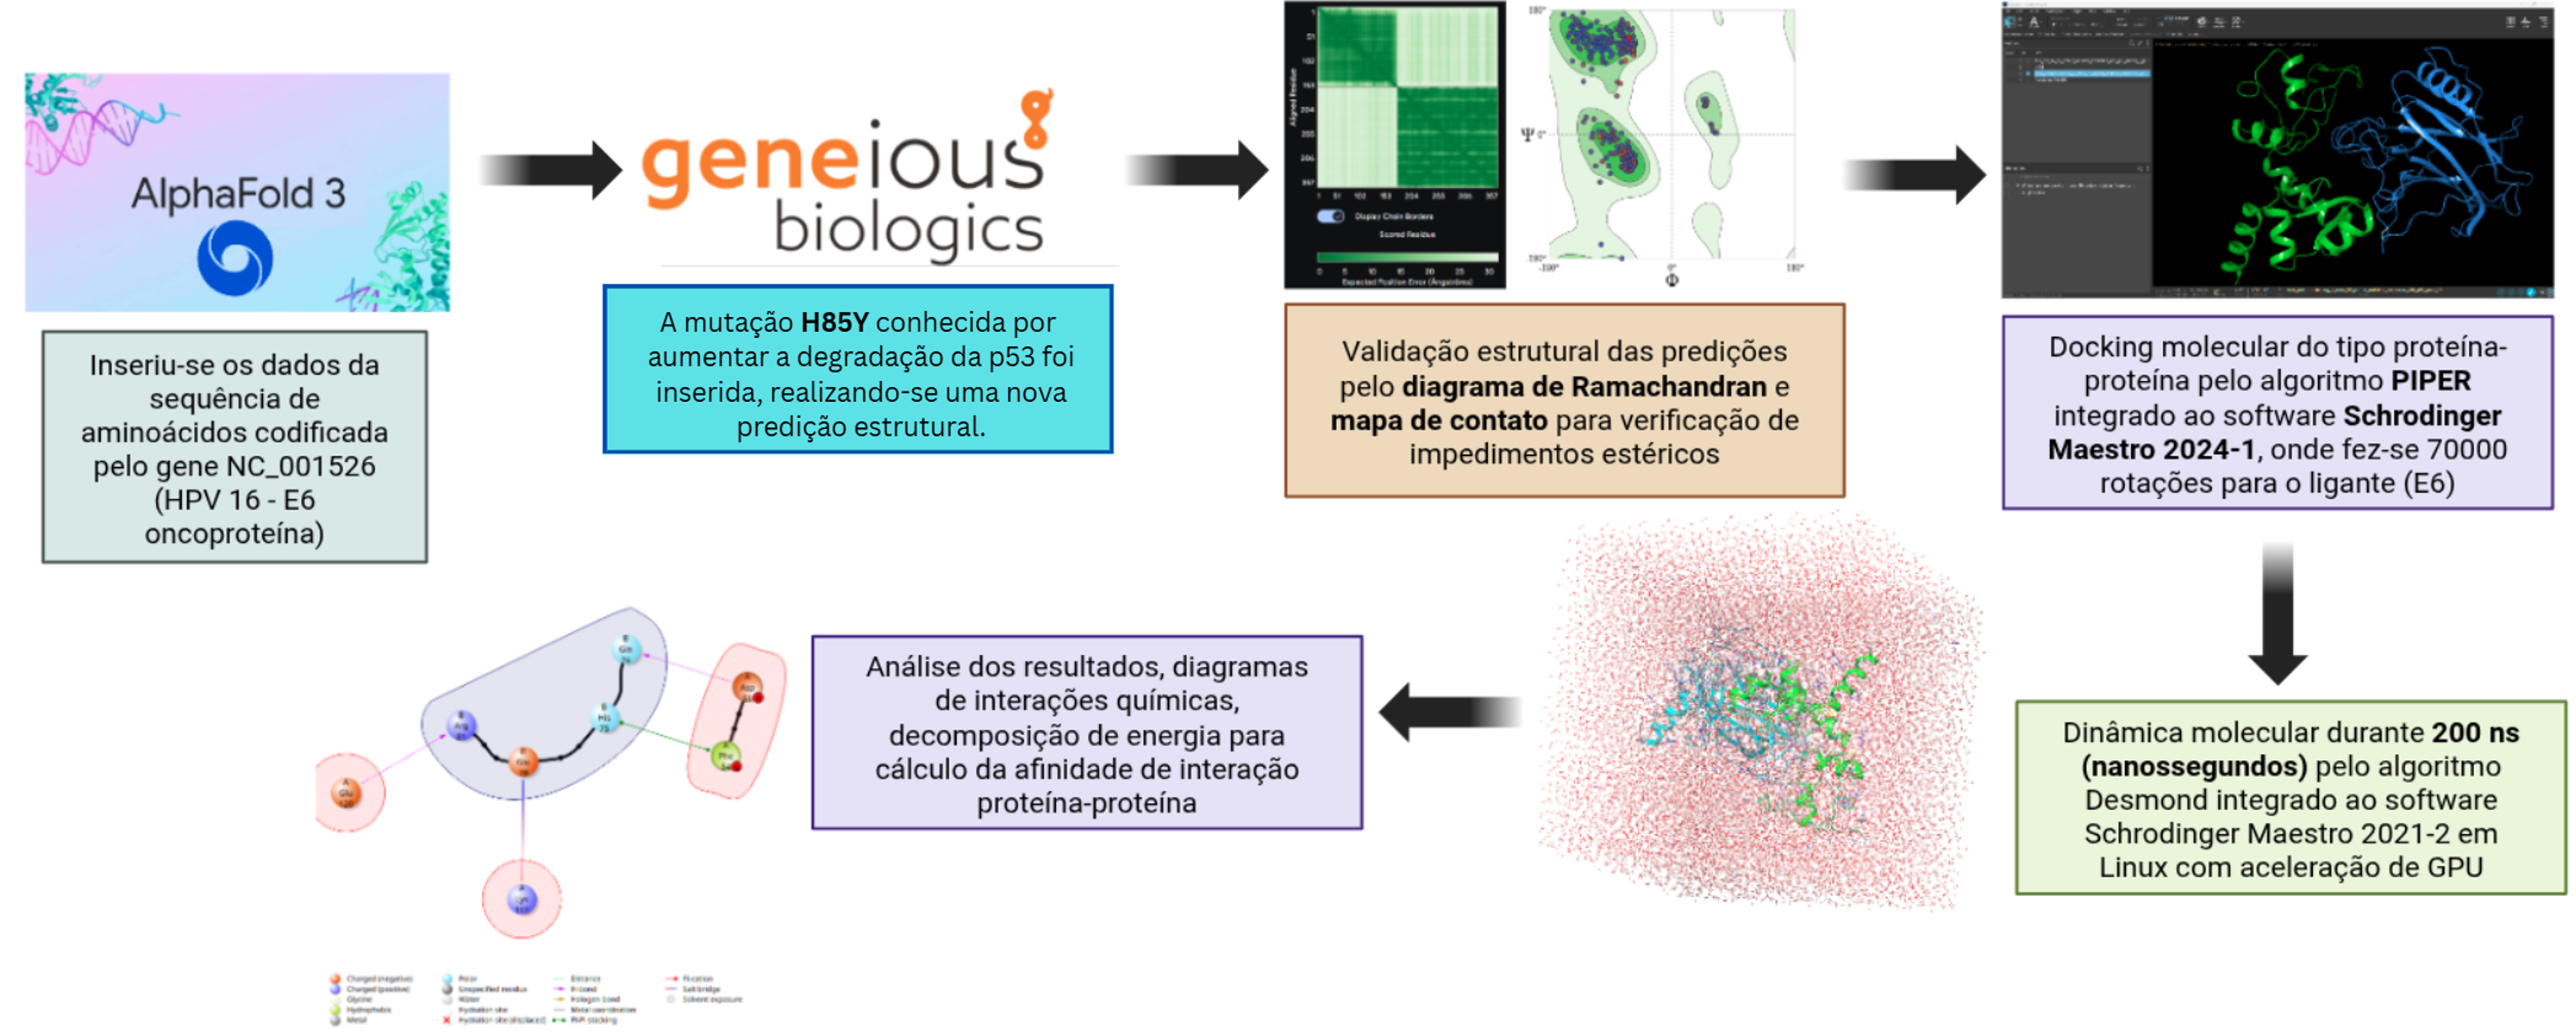
\includegraphics[width=1\linewidth]{Figuras/fluxograma_metodologia.png}
    \caption{Diagrama da metodologia computacional empregada.}
    \label{fig:enter-label}
\end{figure}

\section{Dinâmica molecular na avaliação da estabilidade estrutural}
A partir dos complexos obtidos no docking molecular foi realizado a dinâmica molecular ao longo de 200 ns no software Schrodinger Maestro 2022-1 (Schrödinger, 2022) na sua versão de Linux Ubuntu 24.10 mediante o módulo Desmond com aceleração de GPU RTX 3050. Os parâmetros da simulação foram mantidos a temperatura e pressão constante de 300 K e 1 atm mediante os termostatos de Langevin e barostato de Nosé-Hoover sob o ensemble NPT (número de partículas constante, pressão e temperatura constante). O modelo teórico para as moléculas de água foi o TIP3P com uma caixa de solvatação de geometria cúbica em torno dos complexos. As análises feitas de estabilidade foi principalmente o RMSD (root-mean square deviation) e RMSF (root-mean square fluctuation) ao longo do tempo. Em seguida, foi feito a decomposição de energia MM-GBSA a partir dos últimos 20 ns de simulação para estimativa da afinidade de interação ($\Delta G_{binding}$).

\section{Design de primers para os oncogenes E6/E7}

Serão desenhados um par de primers (Forward e Reverse) que amplifique de forma específica e eficiente uma região conservada dos oncogenes E6 ou E7 do HPV-16, que são os alvos mais comuns para diagnóstico de alto risco. Utilizando-se o software Geneious 11.1.5, fez-se o download do genoma completo do Papilomavírus humano tipo 16 a partir do código de acesso de referência no NCBI GenBank NC\_001526. Após importar, será visualizado a sequência circular do genoma do HPV-16 com suas anotações (genes como E6, E7, L1, L2, etc.) A maioria das reações de PCR (especialmente qPCR), um produto (amplicon) entre 100 e 300 pares de base (pb) é considerado ideal, onde o gene E6/E7 foram selecionado nos quais os primers deverão se anelar. Será utilizado o algoritmo Primer3, que é o padrão-ouro para desenho de primers (UNTERGASSER et al., 2012).

\section{Clonagem e expressão recombinante dos epítopos}

A ferramenta de adaptação de Códons desenvolvida em Java (JCAT) (http://www.prodoric.de/JCat) será utilizada para tradução reversa e otimização de códons de vacinas candidatas projetadas. A otimização de códons será executada para expressar a construção vacinal multiepítopo do vírus HPV-16 em E. coli (cepa K12). Os arquivos de saída serão verificados quanto ao Índice de Adaptação de Códons (IAC) (> 0,8–1,0) e ao conteúdo de GC (30–70\%), para garantir a eficiência transcricional e translacional da construção vacinal projetada. A sequência otimizada de códons resultante das vacinas candidatas será introduzida em sítios específicos. O SnapGene (www.snapgene.com) será finalmente utilizado para inserir a sequência da vacina no vetor de expressão pET-30a(+), entre o sítio de clonagem XhoI e NdeI, obtendo-se os clones finais das vacinas candidatas.

\section{Modelagem da $\beta$-catenina}

As estruturas tridimensionais dos complexos foram modeladas por meio do AlphaFold 3 \cite{Abramson2024} utilizando sequências obtidas no UniProt ($\beta$‑catenina: P35222; TCF4: P15884; BCL9: Q9H1M3; LEF1: Q9NQB0). As interações foram analisadas no PyMOL (Schrödinger, LLC) e avaliadas energeticamente com o servidor PRODIGY \cite{Xue2016}, que fornece valores de energia livre de ligação ($\Delta G$) e constante de dissociação ($K_d$). Foram também
identificados os contatos interfaciais (ICs), classificados em charged–charged, charged–polar, charged–apolar, polar–polar, polar–apolar e apolar–apolar. O perfil de superfície não interfacial (NIS) foi calculado para estimar a proporção de resíduos carregados e apolares.

\chapter{Resultados e Discussões}

Este estudo demonstrou que as mutações encontradas na variante H85Y da oncoproteína E6 do HPV-16 enfraquecem significativamente sua interação com a proteína supressora de tumor p53 em comparação ao wild-type (Figura 2). Essa conclusão é sustentada por uma perda drástica de contatos moleculares: enquanto a forma não mutada do complexo se estabiliza com n ligações de hidrogênio, a variante amazônica mantém apenas n-1 (Figura 3).

\begin{figure}[H]
    \centering
    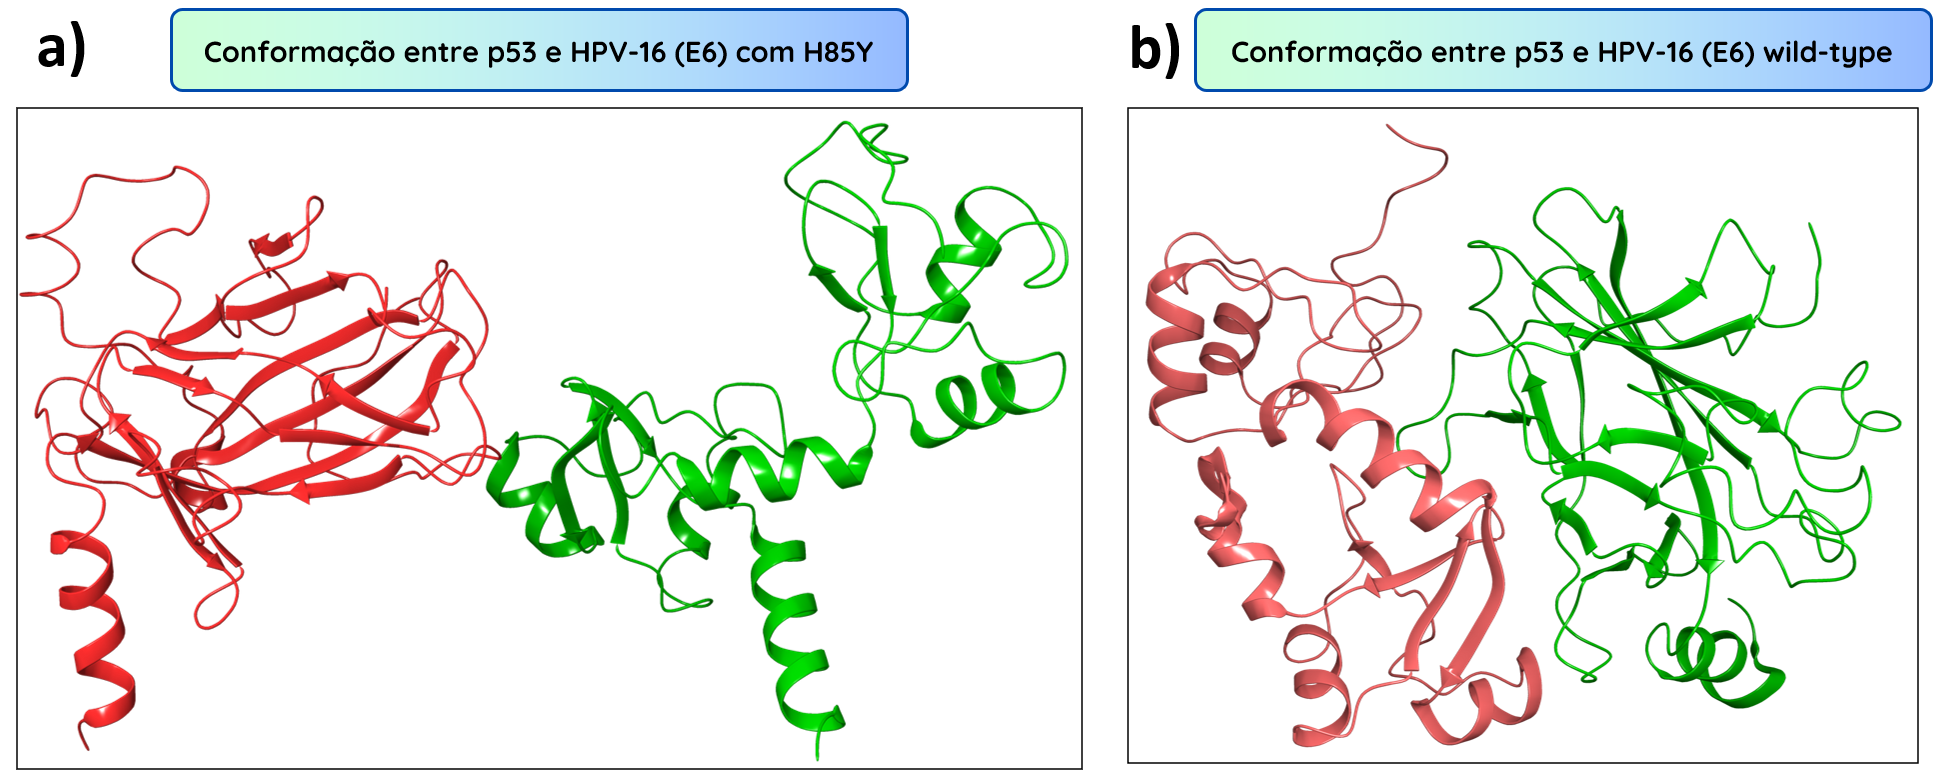
\includegraphics[width=1\linewidth]{Figuras/comparativo_HPV_16_E6_H85_vs_wild_type.png}
    \caption{a) Estrutura tridimensional do frame final após 200 ns de dinâmica molecular da interação entre p53 neutralizando a oncoproteína E6 com a mutação H85Y; b) Estrutura do complexo p53-E6 na forma wild-type, sem mutações; }
    \label{fig:enter-label}
\end{figure}

\begin{figure}[H]
    \centering
    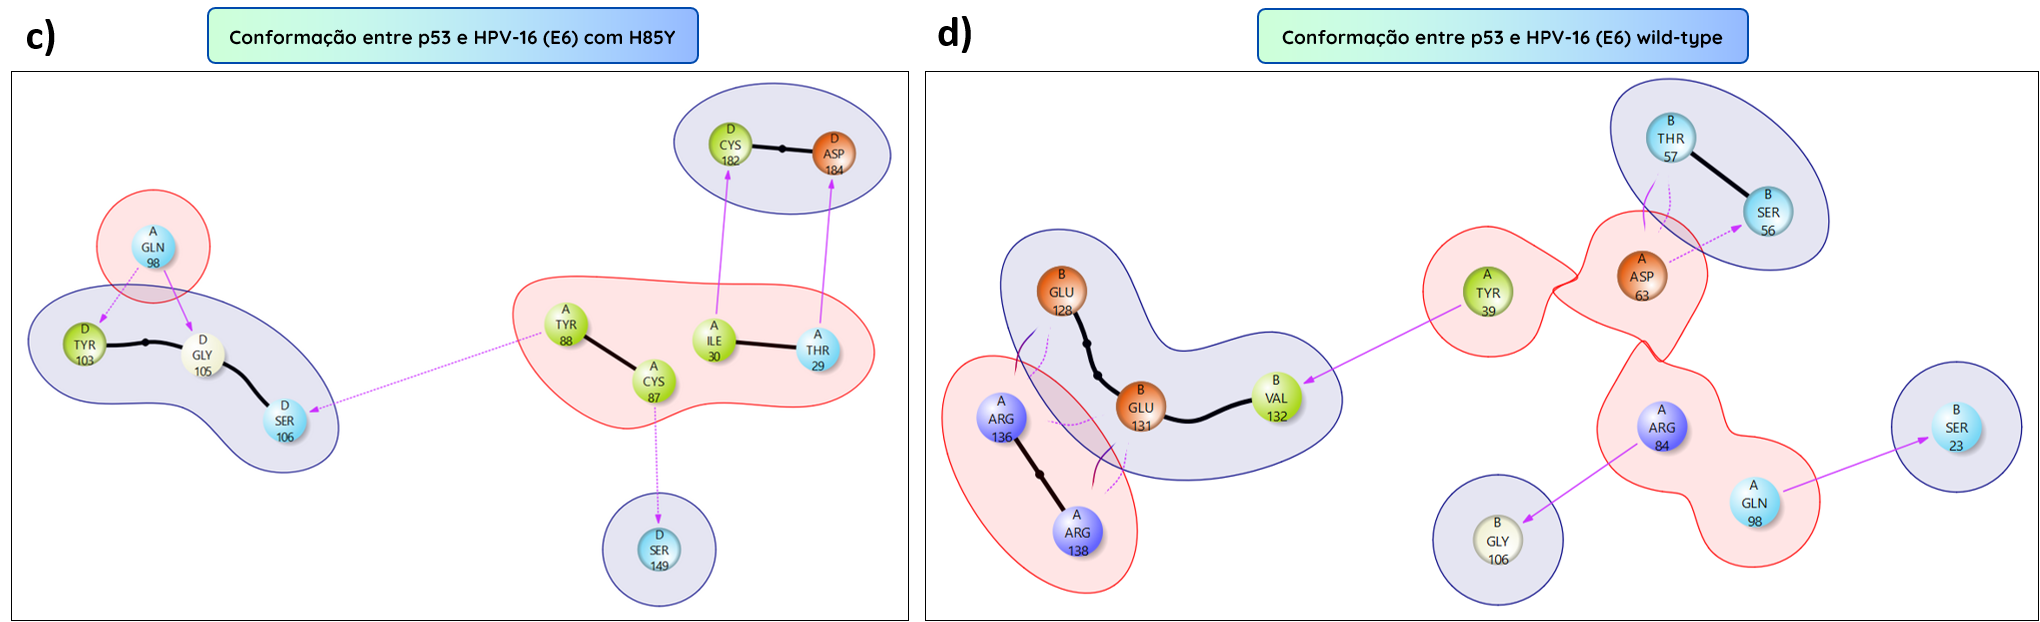
\includegraphics[width=1\linewidth]{Figuras/comparativo_interacoes_HPV_16_E6.png}
    \caption{c) Diagrama de interações para mutação H85Y; d) Diagrama de interações para forma wild-type. }
    \label{fig:enter-label}
\end{figure}


\section{Predição dos epítopos e análise de afinidade}

\begin{table}[H]
    \centering
    \caption{Resultados de afinidade dos epítopos encontrados na interação com receptor de célula T.}
    \begin{tabular}{ccc}
    \hline 
     Sequência    &  $\Delta G$ (kcal/mol)    \\ \hline

    TIHDIILECV  & -42.03 \\
    KLPQLCTEL  & -68. 68 \\ \hline
    \end{tabular}
    \label{tab:my_label}
\end{table}

\section{Predição de miRNA em câncer colorrectal}

\begin{table}[H]
    \centering
    \caption{Resultados de afinidade dos miRNA encontrados na interação com a proteína Argonauta-2.}
    \begin{tabular}{ccc}
    \hline 
     Sequência    &  $\Delta G$ (kcal/mol)    \\ \hline

    mir\_3120\_3p\_2  & -75.14 \\  \hline
    \end{tabular}
    \label{tab:my_label}
\end{table}

\section{Resultado do doking beta-catenina com BCL9, LEF1 e TCF4}

O complexo $\beta$‑Catenina/TCF4 apresentou $\Delta G$ de -26.2 kcal/mol e constante de dissociação ($K_d$) de
$5.9 \times 10^{-20} M$, indicando uma interação de altíssima afinidade. A análise de contatos interfaciais
revelou predominância de interações charged–apolar (95) e charged–polar (49), além de 42
interações charged–charged, demonstrando que a interface é estabilizada por uma combinação de
forças eletrostáticas, hidrofóbicas e de complementaridade estrutural. O perfil de superfície não
interfacial mostrou 23.56\% de resíduos carregados e 43.39\% apolares, sugerindo equilíbrio entre
solubilidade e estabilidade do complexo.

O complexo $\beta$‑Catenina/BCL9 apresentou $\Delta G$ de -37.9 kcal/mol e constante de dissociação
($K_d$) de $1.5 \times 10^{-28} M$, evidenciando uma interação de afinidade ainda mais elevada que a
observada para $\beta$‑catenina/TCF4. A análise de contatos interfaciais indicou predominância
de interações apolar–apolar (136) e charged–apolar (121), complementadas por 48 contatos
charged–charged e 43 charged–polar, configurando uma interface altamente estabilizada
por forças hidrofóbicas e eletrostáticas. O perfil de superfície não interfacial revelou 17.95\% de resíduos carregados e 
51.47\% apolares, reforçando a natureza hidrofóbica dominante do complexo e sua elevada estabilidade conformacional. 
Esses achados destacam o papel crítico de BCL9 como coativador da via Wnt e refletem uma complementaridade estrutural
mais robusta que a observada no complexo $\beta$‑catenina/TCF4.

O complexo $\beta$‑Catenina/LEF1 apresentou $\Delta G$ de -24.0 kcal/mol e constante de dissociação
($K_d$) de $2.4 \times 10^{-18} M$, indicando uma interação de alta afinidade, embora menos intensa do
que as observadas para $\beta$‑catenina/TCF4 e $\beta$‑catenina/BCL9. A análise de contatos
interfaciais revelou predominância de interações charged–apolar (73) e apolar–apolar (59),
além de 42 contatos polar–apolar e 35 charged–charged, sugerindo uma interface
estabilizada principalmente por forças hidrofóbicas, mas com contribuição relevante de
interações eletrostáticas. O perfil de superfície não interfacial apresentou 24.87\% de
resíduos carregados e 43.05\% apolares, indicando equilíbrio entre solubilidade e
estabilidade estrutural. Esses dados reforçam o papel de LEF1 como cofator relevante da
via Wnt, ainda que sua afinidade com a $\beta$‑catenina se apresente inferior àquela observada
para BCL9.

A Tabela 1 resume os resultados obtidos. O complexo $\beta$‑catenina/BCL9 apresentou a maior
afinidade ($\Delta G = -37.9 kcal/mol$; $Kd = 1.5 \times 10^{-28} M$), superando $\beta$‑catenina/TCF4 ($\Delta G =
-26.2 kcal/mol$) e $\beta$‑catenina/LEF1 ($\Delta G = -24.0 kcal/mol$).

\begin{table}[H]
    \centering
    \caption{ Parâmetros energéticos e de contatos interfaciais dos complexos $\beta$‑catenina/TCF4, $\beta$‑catenina/BCL9 e $\beta$‑catenina/LEF1.}
    \begin{tabular}{ccc}
    \hline 
     Interação    & $\Delta G$ (kcal/mol)  & $K_d (M)$   \\ \hline

    $\beta$-Catenina / TCF4 & -26.2 & 5.9 $\times$ 10$^{-20}$  \\
    $\beta$-Catenina / BCL9 & -37.9 & 1.5 $\times$ 10$^{-28}$ \\
   $\beta$-Catenina / LEF1 & -24.0 & 2.4 $\times$ 10$^{-18}$  \\ \hline
    \end{tabular}
    \label{tab:my_label}
\end{table}

A análise mostra que a interação $\beta$‑catenina/BCL9 é mais estável e fortemente guiada por
contatos hidrofóbicos (AA e CA), indicando que essa interface é crítica para a manutenção
da sinalização Wnt. Já o complexo $\beta$‑catenina/TCF4 apresentou predominância de
interações eletrostáticas (CC e CP), reforçando seu papel de especificidade na transcrição
gênica. O complexo $\beta$‑catenina/LEF1, com afinidade intermediária, combina contatos
hidrofóbicos e eletrostáticos, sugerindo que pode atuar como regulador adicional, mas
menos dominante que BCL9. Esses achados são consistentes com a literatura, que aponta
BCL9 como um dos principais coativadores da via Wnt em tumores avançados.

Os resultados obtidos permitem uma análise comparativa da afinidade e estabilidade
estrutural dos complexos da $\beta$‑catenina com três parceiros-chave da via Wnt: TCF4, BCL9 e
LEF1.

O complexo $\beta$‑catenina/BCL9 apresentou a maior afinidade ($\Delta G = -37.9 kcal/mol$;
$K_d = 1.5 \times 10^{-28} M$), superando $\beta$‑catenina/TCF4 e $\beta$‑catenina/LEF1.

A elevada contribuição de interações apolar–apolar (136) sugere que BCL9 exerce
papel crítico na estabilização prolongada do complexo.

Já $\beta$‑catenina/TCF4, apesar de menor $\Delta G$, mantém alta relevância funcional devido
à sua predominância de interações eletrostáticas (charged–polar e
charged–charged), o que favorece a especificidade no reconhecimento.

$\beta$‑catenina/LEF1 apresentou afinidade intermediária, com equilíbrio entre contatos
hidrofóbicos e eletrostáticos, reforçando sua função como modulador, mas
possivelmente com papel menos dominante que BCL9 e TCF4.
Implicações funcionais:

O predomínio de interações hidrofóbicas no complexo $\beta$‑catenina/BCL9 sugere que
a sua interrupção poderia desestabilizar significativamente a sinalização Wnt, sendo
um alvo estratégico.

O complexo $\beta$‑catenina/TCF4, essencial para a transcrição gênica, permanece como
alvo clássico, mas pode demandar abordagens que preservem a seletividade para
evitar toxicidade.

LEF1, embora com afinidade menor, pode atuar em redundância com TCF4,
sugerindo que terapias combinadas visando múltiplas interfaces podem ser mais
eficazes.

A identificação de $\Delta G$ e perfis de interação fornece subsídios para o
desenvolvimento de peptídeos miméticos ou pequenas moléculas inibidoras capazes
de competir com TCF4, BCL9 ou LEF1 pela ligação à $\beta$‑catenina.

O bloqueio específico da interface $\beta$‑catenina/BCL9 surge como promissora
estratégia, dada sua afinidade superior, podendo resultar em maior supressão da via
Wnt em contextos tumorais. No entanto, o equilíbrio observado em LEF1 e TCF4 sugere que abordagens
multitarget podem prevenir mecanismos de escape celular. Estudos futuros devem avaliar não apenas a afinidade estática, mas também a dinâmica conformacional e a viabilidade farmacológica de candidatos, ampliando o potencial de translação clínica dos achados.